\subsection{Limitaciones de los actuadores}

\subsubsection{Limitaciones del servomotor}

El servomotor recibe una señal tipo PWM, cuyo ancho de pulso determina el ángulo al cual se moverá. Según su hoja de datos, un ancho de pulso de \qty{1}{\ms} se corresponderá con un ángulo de \qty{-90}{\degree}, mientras que un ancho de pulso de \qty{2}{\ms} se corresponde con un ángulo de \qty{90}{\degree}. Por otro lado, se especifica que la mínima resolución temporal que presenta el servo es de \qty{5}{\us}, lo que resulta en
$$\frac{\qty{2}{\ms} - \qty{1}{\ms}}{\qty{5}{\us}} = 200$$
incrementos. Dado que la amplitud total es de \qty{180}{\degree}, resulta que la resolución angular del servomotor es de \qty{0.9}{\degree}.

Se realizaron experimentos con el servo y se encontró que el rango de tiempos que obtiene la excursión angular completa es de \qtyrange{600}{2400}{\us}. Sin embargo, consideramos como peor caso que sigue habiendo 200 incrementos angulares, en lugar de recalcular la resolución contemplando los \qty{5}{\us} especificados.

Además, contemplando que la biblioteca \verb|Servo.h| utilizada para comandar al motor emplea un temporizador de \qty{16}{\bit} para generar la señal PWM, la cantidad de divisiones de un período de la señal será de $2^{16} = 65536$. Como la frecuencia es de \qty{50}{\Hz}, su período es de \qty{20}{\ms}. Entonces, la resolución temporal que se obtiene con el temporizador es de
$$\frac{\qty{20}{\ms}}{2^{16}} = \qty{305}{\ns}.$$
Como este valor es menor a la resolución temporal del servo, consideramos que la limitación está dada por el servomotor y la resolución angular es la calculada anteriormente,
$$\Delta\theta = \qty{0.9}{\degree}.$$

Dado que el servomotor se utilizará para mover la barra, es necesario conocer cómo el giro del servo afecta al ángulo de la barra. La Figura~\ref{fig:angulo-barra} muestra un modelo simplificado del sistema servo-barra. Si suponemos que la barra vertical del brazo solo presenta rotaciones muy pequeñas respecto de la vertical, entonces podemos aproximar $x \approx x'$, de donde se obtiene la siguiente relación:
\begin{align*}
    L \sin(\alpha) = l \sin(\theta),
\end{align*}
y por lo tanto tendremos que
\begin{align*}
    \alpha = \sin^{-1}\left(\frac{l}{L} \sin(\theta)\right).
\end{align*}

\begin{figure}[!tbp]
    \centering
    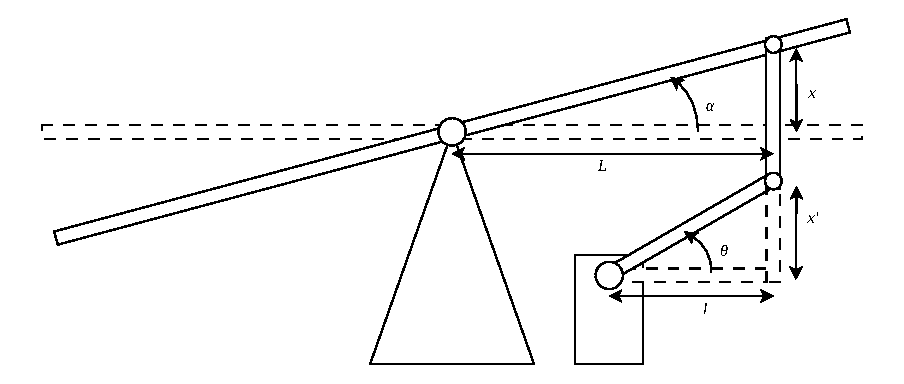
\includegraphics[width=\linewidth]{barra-angulo}
    \caption{Modelo simplificado del sistema servo-barra.}
    \label{fig:angulo-barra}
\end{figure}

Las longitudes involucradas toman los siguientes valores: $L = \qty{10.5}{\cm}$ y $l = \qty{4.5}{\cm}$. La relación resultante es de $\alpha = 0.429$. Para calcular la mínima resolución angular que se puede comandar a la barra, utilizamos la aproximación de ángulos pequeños, resultando en
\begin{align*}
    \Delta\alpha \approx \frac{l}{L} \Delta \theta = \qty{0.4}{\degree}.
\end{align*}
Por ende, se consigue en el comando de la barra una resolución mejor que la que intrínsecamente posee el servomotor.

Para corroborar experimentalmente el cálculo anterior, se comandaron diferentes ángulos al servomotor y se midió utilizando el acelerómetro el çangulo resultante en la barra. El Cuadro~\ref{tab:angulos} muestra lo ángulos comandados al servomotor, el ángulo medido en la barra, y el cociente de los primeros sobre los últimos, que se corresponden con el valor de $\alpha$. Vemos que hay cierta dispersión en los valores medidos, pero en promedio se obtiene un $\alpha = 0.390$ experimental, lo que representa una diferencia del \qty{9.1}{\percent} respecto del valor teórico. Se considera el error aceptable, y se tomará la relación medida ($\alpha = 0.39$) para el desarrollo de los siguientes trabajos.

% Promedio 0.390

\begin{table}[!tbp]
    \centering
    \begin{tabular}{SSS}
        \toprule
        {Ángulo del servo [\unit{\degree}]} & {Ángulo de la barra [\unit{\degree}]} & {$\alpha$} \\
        \midrule
        -30.0 & -11.6 & 0.387 \\
         30.0 &  11.4 & 0.380 \\
        -20.0 & -8.0  & 0.400 \\
         20.0 &  7.7  & 0.385 \\
        -10.0 & -4.1  & 0.410 \\
         10.0 &  3.8  & 0.380 \\
        \bottomrule
    \end{tabular}
    \caption{Ángulos comandados al servo y resultantes en la barra.}
    \label{tab:angulos}
\end{table}

% TODO: Estimar tiempo requerido para mover el servo 30 grados
% TODO: Recalcular todo para frecuencia de 1 Hz

% vim: ts=4 sts=4 sw=4 et lbr
